\documentclass[handout]{beamer}

\usepackage{beamerthemesplit}
\usepackage{pgfpages}
\usepackage{verbatim}
\usepackage{fancybox}

%\usepackage{algorithmic}
\usepackage{amsmath}
\usepackage{amsthm}
\usepackage{algorithm2e}
\usepackage{algorithmic}
\usepackage{lipsum}% http://ctan.org/pkg/lipsum
\usepackage{xifthen}% http://ctan.org/pkg/xifthen
\usepackage{needspace}% http://ctan.org/pkg/needspace
\usepackage{hyperref}% http://ctan.org/pkg/hyperref

\newcommand{\field}[1]{\mathbb{#1}} %requires amsfonts

% Multiple pages...
%\pgfpagesuselayout{4 on 1}

\usetheme{Antibes}
\usecolortheme{beaver}
\title[Team Satisfaction - $3$-$SAT$]{The $3$-$SAT$ Decision Problem \\ Exhaustive Search Implementations}

\usepackage{mathptmx}
\usepackage[scaled=.90]{helvet}
\usepackage{courier}
\usepackage[T1]{fontenc}

%\pgfpagesuselayout{4 on 1}[letterpaper,border shrink=5mm]

\institute[RIT]{}
\date{\today}
\subtitle{Team Satisfaction}
\author{Christopher Wood, Eitan Romanoff, Ankur Bajoria}
%\institute[]{}
\date{\today}

\begin{document}

\begin{frame}
	\titlepage
\end{frame}

\begin{frame}
	\frametitle{Agenda}
	\tableofcontents
\end{frame}

\section{Problem Statement}
\begin{frame}
	\frametitle{Boolean Satisfiability}

	Boolean satisfiability is an $NP$-complete decision problem defined as:
	\begin{align*}
	SAT : \phi \to \{YES, NO\}
	\end{align*}

	\medskip

	\textbf{Input}: Boolean formula $\phi$ on $n$ variables.

	\medskip 

	\textbf{Output}: $YES$ if there exists a variable truth assignment to the
	variables in $\phi$ such that it evaluates to true, $NO$ otherwise.

	\medskip

	\begin{center}
		$\phi$ is satisfiable $\Leftrightarrow$ $SAT(\phi) = YES$
	\end{center}

\end{frame}

% TODO: give a sample circuit of the problem

\begin{frame}
	\frametitle{$3$-$SAT \in NP$}
	\begin{itemize}
		\item A special case of $SAT$ that fixes the format of $\phi$.
		\item Each input formula is in $3$-$CNF$ form:
		\begin{itemize}
			\item The conjunction (Boolean AND) of arbitrarily many clauses, 
			where each clause is the disjunction (Boolean OR) of exactly three literals 
			(a Boolean variable or its negation).

			\begin{align*}
				(x_1 \lor x_2 \lor \lnot x_3) \land (x_1 \lor x_2 \lor x_3) \land (x_1 \lor x_2 \lor x_3)
			\end{align*}

		\end{itemize}
		\item $SAT$ reduces to $3$-$SAT$, so $3$-$SAT \in NP$.
	\end{itemize}
\end{frame}

% TODO: give example of 3-CNF formula

\section{Exhaustive Search Algorithm}
\begin{frame}[fragile]
	\frametitle{Exhaustive Search for $3$-$SAT$}
	% DESCRIBE exhaustive search algorithm for this problem
	% (in pseudocode)
	
\textbf{Input:} $3$-$CNF$ formula $\phi_n$ on $n$ variables, \textbf{Output:} YES or NO 

\medskip

\begin{algorithm}[H]
\begin{algorithmic}[1]
\STATE $C \gets FALSE^n$ (vector of $n$ False values, the initial configuration)
\FOR{$i = 0 \to 2^n - 1$}
	\STATE $SAT \gets TRUE$
	\FORALL{$clause \in \phi_n$}
		\IF{$evaluate(clause, C) = FALSE$}
			\STATE $SAT \gets FALSE$
		\ENDIF
	\ENDFOR	
	\STATE \textbf{if} $SAT = TRUE$ \textbf{then return} $YES$
	\STATE $C \gets nextConfig(C)$
\ENDFOR
\RETURN $NO$
\end{algorithmic}
%\caption{Exhaustive search for $3$-$SAT$.}
\label{alg:seq}
\end{algorithm}
	
%	input: 
%	for each $2^n$ variable configuration
%		assign variable to literals in $\phi$ 
%		evaluate $\phi$
%		if (true) return YES
%	return NO
\end{frame}

\begin{frame}[fragile]
	\frametitle{Evaluating a Clause}
\begin{itemize}
	\item Evaluating a clause depends on how $\phi_n$ and the variable truth assignments are stored.
	\begin{itemize}
		\item {\tt boolean[]} for variable assignments and {\tt Literal[][3]} for $\phi_n$.
	\end{itemize}
	\item A literal is true (meaning the clause is true), if one of the following hold:
	\begin{itemize}
		\item The literal is negated and its assignment is false.
		\item The literal is not negated and its assignment is true.
	\end{itemize}
	\item Two (fast) lookups and Boolean operations.
\end{itemize}
\end{frame}

\begin{frame}
	\frametitle{Exhaustive Search for $3$-$SAT$ - A \emph{Very Satisfiable} Example!}
\textbf{Input}: $\phi_5 = (\lnot X_1 \lor \lnot X_2 \lor \lnot X_3) \land (X_3 \lor \lnot X_4 \lor \lnot X_5)$ \\
\textbf{Output}: Yes \\ 
\textbf{Note}: no early termination once a satisfiable solution is found
\begin{figure}
\centering
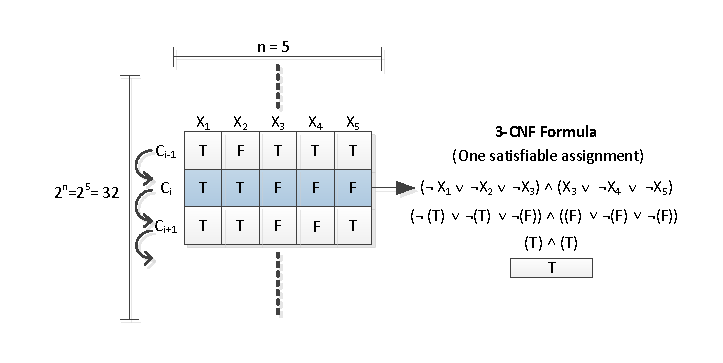
\includegraphics[scale = 0.8]{satSolverAlg.pdf}
\end{figure}
	% image of how the algorithm works 
	% Array of truth values on left, arrows that point to literals, and then output truth value on the right
\end{frame}

\section{Sequential Program Demo}
\begin{frame}
	\frametitle{The Sequential Solver}
	\begin{center}
		Demo time!
		\begin{align*}
			\phi_5 = (\lnot X_1 \lor \lnot X_2 \lor \lnot X_3) \land (X_3 \lor \lnot X_4 \lor \lnot X_5)
		\end{align*}
	\end{center}
\end{frame}

%\begin{frame}
%	\frametitle{References}
%	\bibliographystyle{plain}
%	\bibliography{authenticated_encryption}
%\end{frame}

\begin{comment}
\begin{figure}
\centering
\includegraphics[scale = 0.6]{images/sub_layer.jpg}
\end{figure}
\end{comment}

\end{document}
